\documentclass[12pt]{article}
\usepackage{graphicx} % Required for inserting images
\usepackage{float}
\usepackage{listings}
\usepackage[dvipsnames]{xcolor}
\usepackage{geometry}
\usepackage[UTF8]{ctex}
\usepackage{amsmath}


\title{Pre-lecture Problems for Lecture 3:\\ Integer Programming}
\author{B10705034 資管三\ 許文鑫}
\geometry{a4paper,scale=0.8}
\begin{document}
\maketitle
\begin{enumerate}
      \item (0 point) Consider the following integer
            program
            \begin{align*}
                  \text{max }  & x_1 + x_2                      \\
                  \text{s.t. } & 2x_1 + x_2 - 6 \leq M_1z       \\
                               & x_1 + 2x_2 - 8 \leq M_2(1-z)   \\
                               & x_1 \leq 10                    \\
                               & x_2 \leq 10                    \\
                               & x_i \geq 0 \ \ \forall i = 1,2 \\
                               & z \in \{0,1\},
            \end{align*}
            where $M_1$ and $M_2$ are parameters and $x_1$, $x_2$, and $z$ are variables. The binary variable $z$ is to select at least one constraint to be satisfied.
            \begin{enumerate}
                  \item What values of $M_1$ and $M_2$ can enable $z$ to do the "at-least-one" selection?\\
                        \textbf{Ans. }
                        $M_1 = 24, M_2 = 22$
                  \item Depict the feasible region on the $(x_1,x_2)$ plane. Then graphically solve the IP.\\
                        \textbf{Hint.} The feasible region is nonconvex on the $(x_1,x_2)$ plane. To solve this problem graphically, no branch-and-bound is needed.\\
                        \textbf{Ans. }\\
                        $x_1= 8,x_2=0$
                        \begin{figure}[H]
                              \centering
                              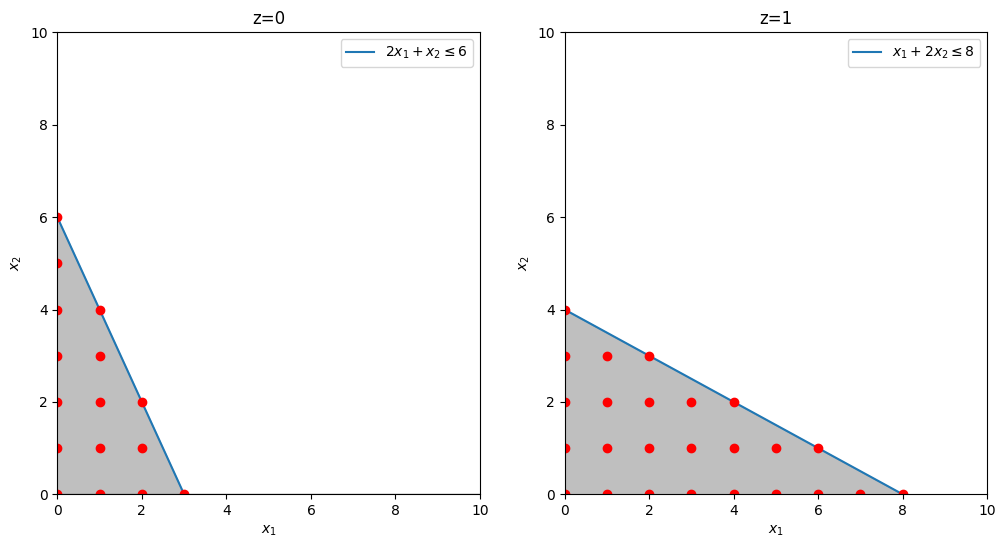
\includegraphics[width=0.4\textwidth]{p1.png}
                        \end{figure}
            \end{enumerate}
      \item (0 point) Six towns locate at the following six points on a Cartesian plane: $(0, 60)$, $(20, 50)$, $(30, 20)$, $(40,80)$, $(50,50)$, and $(90,60)$ (in km). Currently a company owns six retail stores, one in each town. The weekly sales of a product in these stores are $10000$, $15000$, $12000$, $8000$, $20000$, and $3000$. The company currently has one distribution center (DC) in town $3$. It plans to build some more DCs for the retail stores to replenish from. The construction costs of building a DC in these towns are $\$200000$, $\$180000$, $\$160000$, $\$190000$, $\$150000$, and $\$200000$. A truck can carry 500 units of this product. The shipping cost for a truck to move $1$ km is $\$1$. The existing DC and any newly built DC can be used for $5$ years. There is no capacity limit for a DC. Transportation between two locations can be done by traveling through the straight line connecting them.
            \begin{enumerate}
                  \item Formulate the problem of minimizing the $5$-year total construction and shipping costs as an integer program if DCs can only be built in towns.\\
                        \textbf{Ans. }
                        Let $x_{ij}$ be the amount of product shipped from town $i$ to town $j$, and $y_i$ be the binary variable indicating whether a DC is built in town $i$, $c_{ij}$ be the distance between town $i$ and $j$, $c_i$ be the costs of building a DC in town $i$, $s_j$ be the weekly sales of a product in the store of town $j$. Then the integer program is
                        \begin{align*}
                              \text{min }  & \sum_{i=1}^{6} \sum_{j=1}^{6} c_{ij}\times \lceil \frac{x_{ij}}{500}\rceil + \sum_{i=1}^{6} y_i c_i \\
                              \text{s.t. } & \sum_{i=1}^{6} x_{ij} \geq s_j \ \ \forall j = 1,2,3,4,5,6                                          \\
                                           & y_i \in \{0,1\} \ \ \forall i = 1,2,3,4,5,6
                        \end{align*}
                  \item Suppose DCs may also be built in the following locations: $(0, 20)$, $(20, 40)$, $(40, 30)$, and $(60, 40)$. Do Part (a) again.
                  \item
            \end{enumerate}
      \item (10 point; 5 points each) Ten jobs should be scheduled on one single machine. The processing times for these jobs are $7, 4, 3, 9, 10, 6, 8, 9, 7, \text{ and } 10$ (in hours). The due times for these jobs are $40, 43, 45, 46, 49, 50, 52, 57, 58, \text{ and } 60$ (in hours).
            \begin{enumerate}
                  \item Suppose that we want to minimize the total \textbf{\textit{tardiness}} of all jobs. For a job, its tardiness is its completion time minus its due time if this quantity is positive or zero otherwise. For the schedule (1,2,3,4,5,6,7,8,9,10), which means first processing job 1, then job 2 right after job 1 is done, then job 3 right after job 2 is done, etc., calculate the total tardiness.\\
                        \textbf{Ans. }\\
                        The completion time of these job is $7,11,14,23,33,39,47,56,63,73$, and the tardiness of these job is $0,0,0,0,0,0,0,0,5,13$, so the total tardiness is $18$.
                  \item Formulate an integer program that finds a schedule to minimize the total tardiness of all jobs.\\
                        \textbf{Ans. }\\
                        Let $w_j$ be the amount of tardiness of job $j$, $p_j$ be the processing time of job $j$, $d_j$ be the due time of job $j$, $x_j$ be the ocmpletion time of job $j$. Then the integer program is
                        \begin{align*}
                              \text{min }  & \sum_{j=1}^{10} w_j                                                                    \\
                              \text{s.t. } & w_j \geq 0         \ \ \forall j = 1,2, ..., 10                                        \\
                                           & w_j \geq x_j - d_j \ \  \forall j=1,2, ...,10                                          \\
                                           & x_j \geq p_j   \ \ \forall j = 1,2, ..., 10                                            \\
                                           & x_j \geq 0     \ \ \forall j = 1,2, ..., 10                                            \\
                                           & x_i+p_j - x_j \leq Mz_{ij} \ \ \forall j = 1,2,...10, \forall i = 1,2,...,10, i<j      \\
                                           & x_j + p_i - x_i \leq M(1-z_{ij})\ \ \forall j = 1,2,...10, \forall i = 1,2,...,10, i<j \\
                                           & z_{ij} \in \{0,1\} \ \ \forall j = 1,2,...10, \forall i = 1,2,...,10, i<j
                        \end{align*}
            \end{enumerate}
\end{enumerate}
\end{document}